
\documentclass[10pt,a4paper]{article}
\usepackage{f1000_styles}

%% Default: numerical citations
% \usepackage[numbers]{natbib}

%% Uncomment this lines for superscript citations instead
% \usepackage[super]{natbib}

%% Uncomment these lines for author-year citations instead
% \usepackage[round]{natbib}
% \let\cite\citep

%% lines required to use a CSL style for references

%% lines to get the code chunks working

%% lines to enable bulletpoints in a new notation style
\providecommand{\tightlist}{%
  \setlength{\itemsep}{0pt}\setlength{\parskip}{0pt}}

\begin{document}
\pagestyle{fancy}

\title{Applying a Multiverse to Population Habitat Analyses}
\author[1]{Benjamin Michael Marshall*}
\author[1]{Alexander Bradley Duthie**}
\affil[1]{Biological and Environmental Sciences, Faculty of Natural Sciences, University of Stirling, Stirling, FK9 4LA, Scotland, UK}

\affil[*]{\href{mailto:benjaminmichaelmarshall@gmail.com}{\nolinkurl{benjaminmichaelmarshall@gmail.com}}}
\affil[**]{\href{mailto:alexander.duthie@stir.ac.uk}{\nolinkurl{alexander.duthie@stir.ac.uk}}}

\maketitle
\thispagestyle{fancy}

\begin{abstract}

abc

\end{abstract}

\section*{Keywords}

Movement ecology, simulation, compana, resource selection functions, step selection function, habitat preference, habitat selection, animal movement, multiverse, research choice, researcher degrees for freedom,

\clearpage
\pagestyle{fancy}

\hypertarget{introduction}{%
\section{Introduction}\label{introduction}}

abc

\hypertarget{methods}{%
\section{Methods}\label{methods}}

test
test

\hypertarget{results}{%
\section{Results}\label{results}}

\hypertarget{specification-curves}{%
\subsection{Specification Curves}\label{specification-curves}}

(Fig. \ref{fig:specCurveArea}).

\begin{figure}
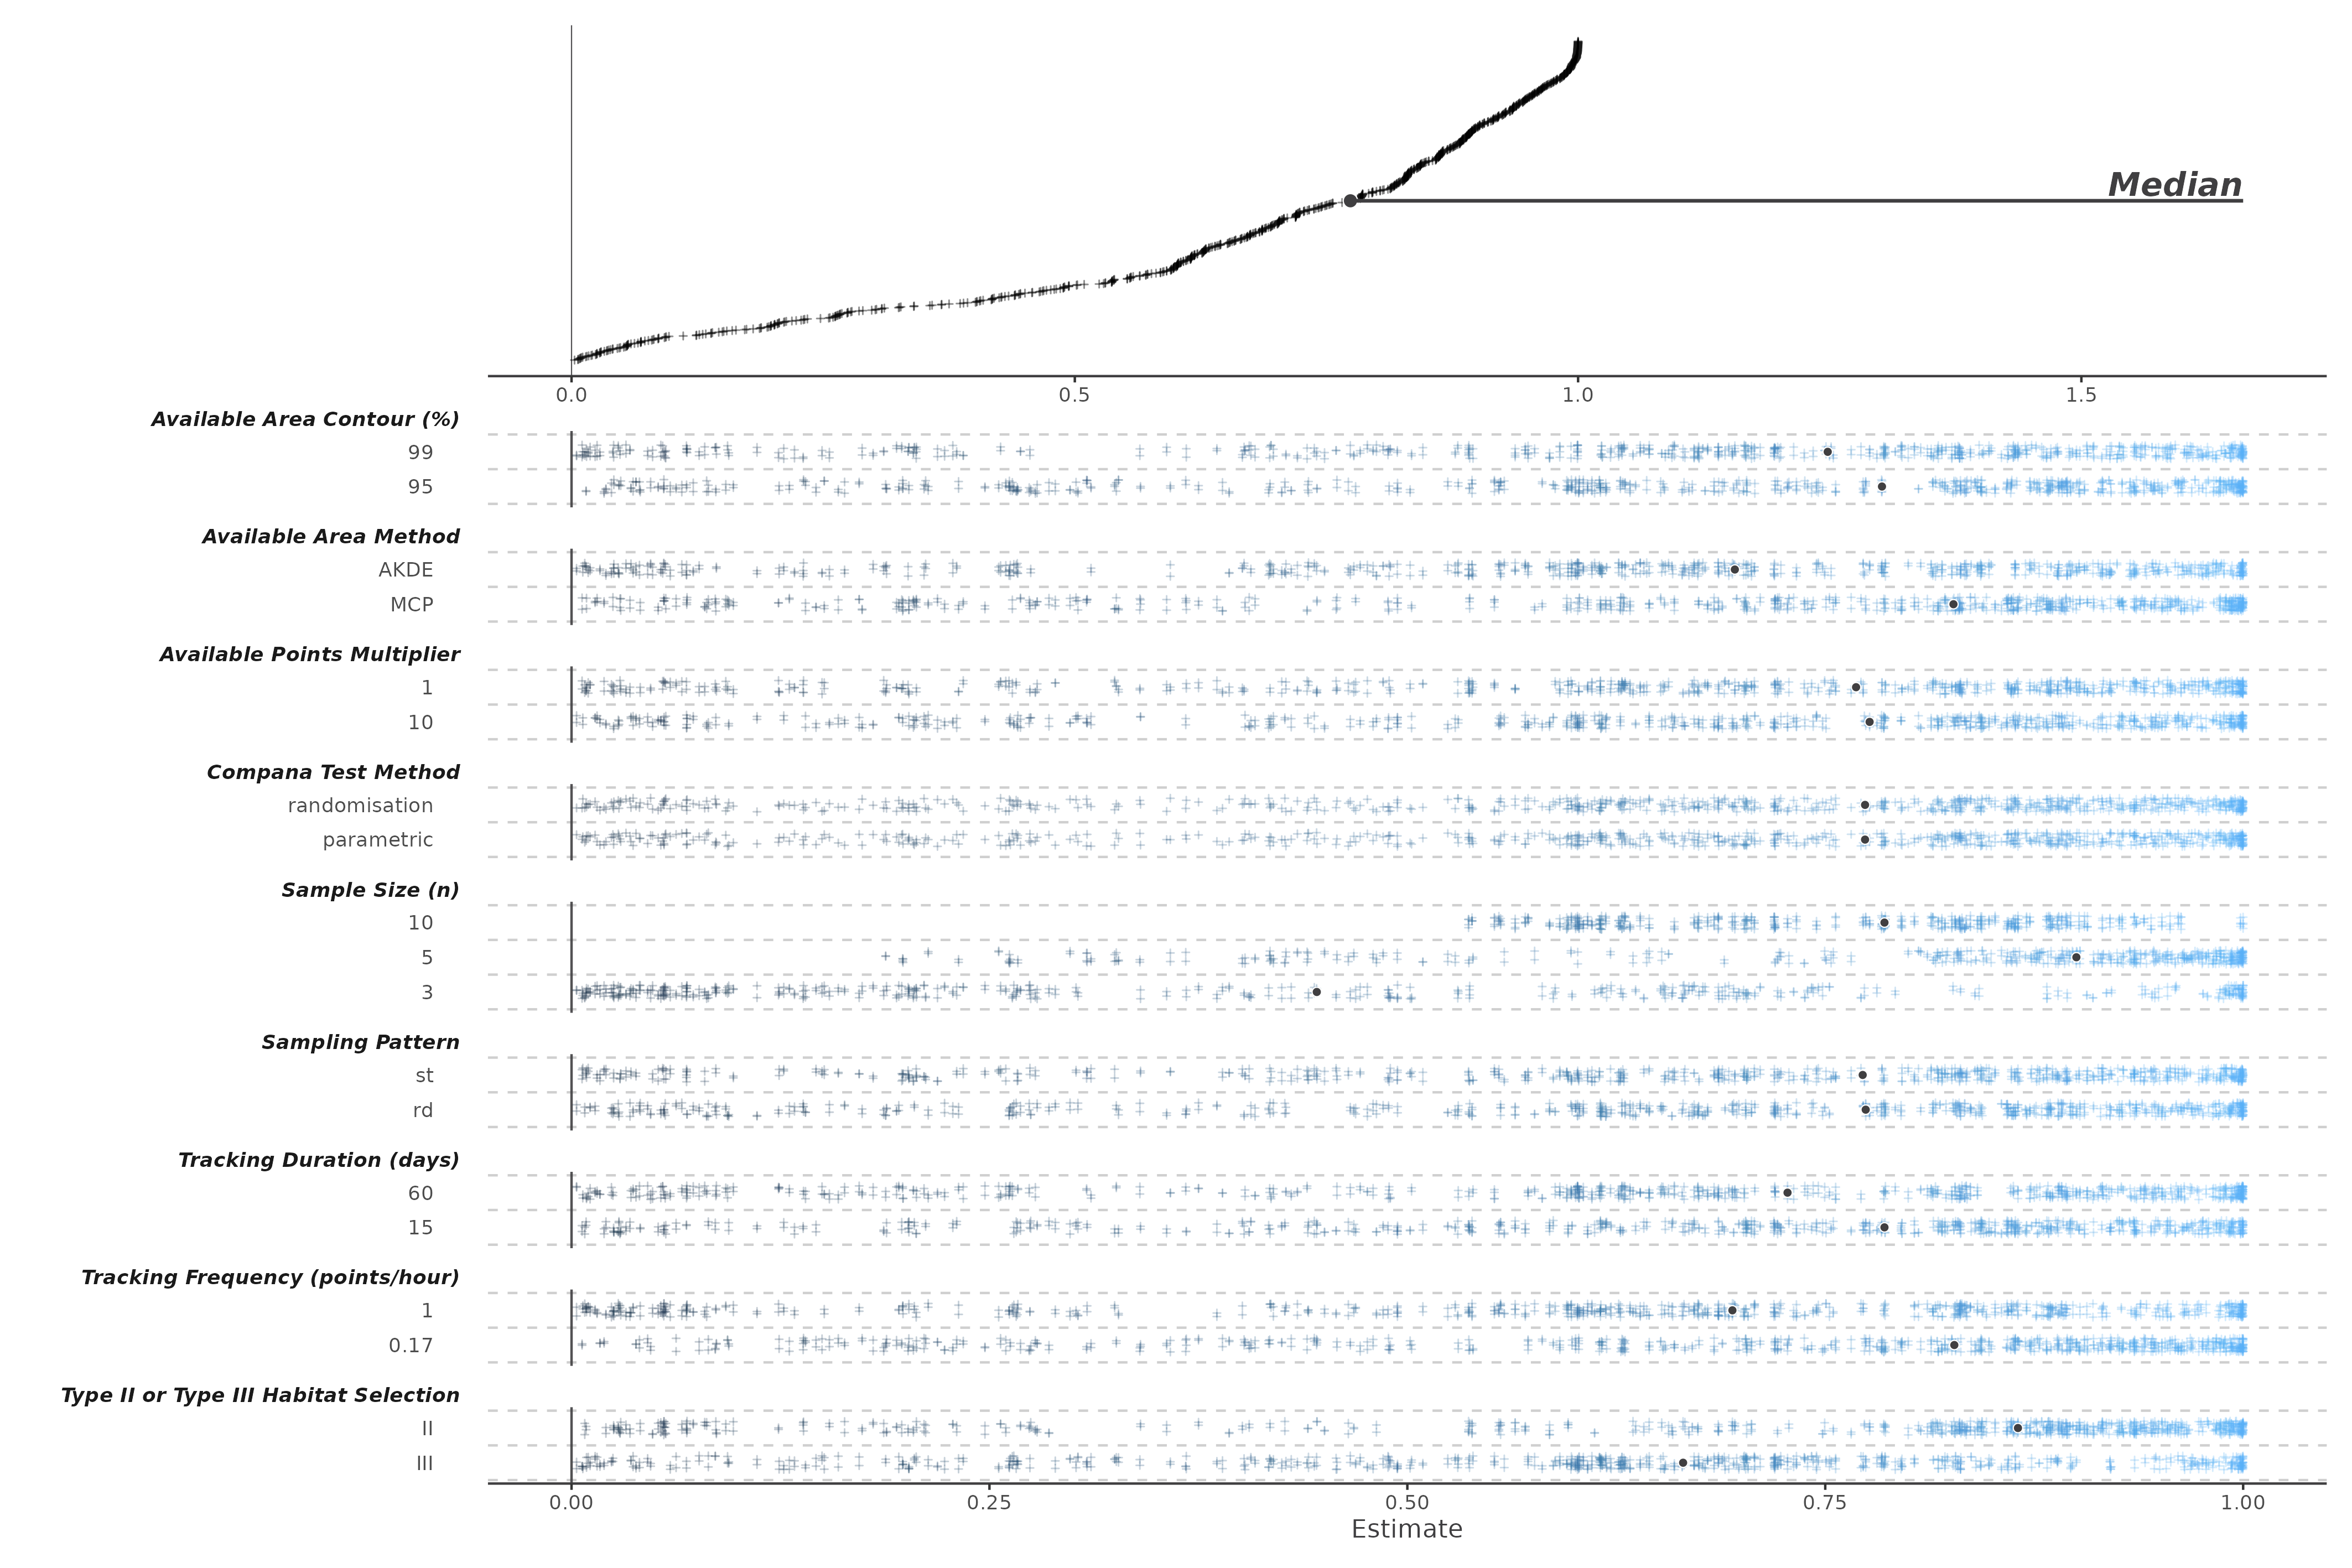
\includegraphics[width=1\linewidth]{../figures/area_specCurve} \caption{Spec curve}\label{fig:specCurveArea}
\end{figure}

(Fig. \ref{fig:specCurveSSF}).

\begin{figure}
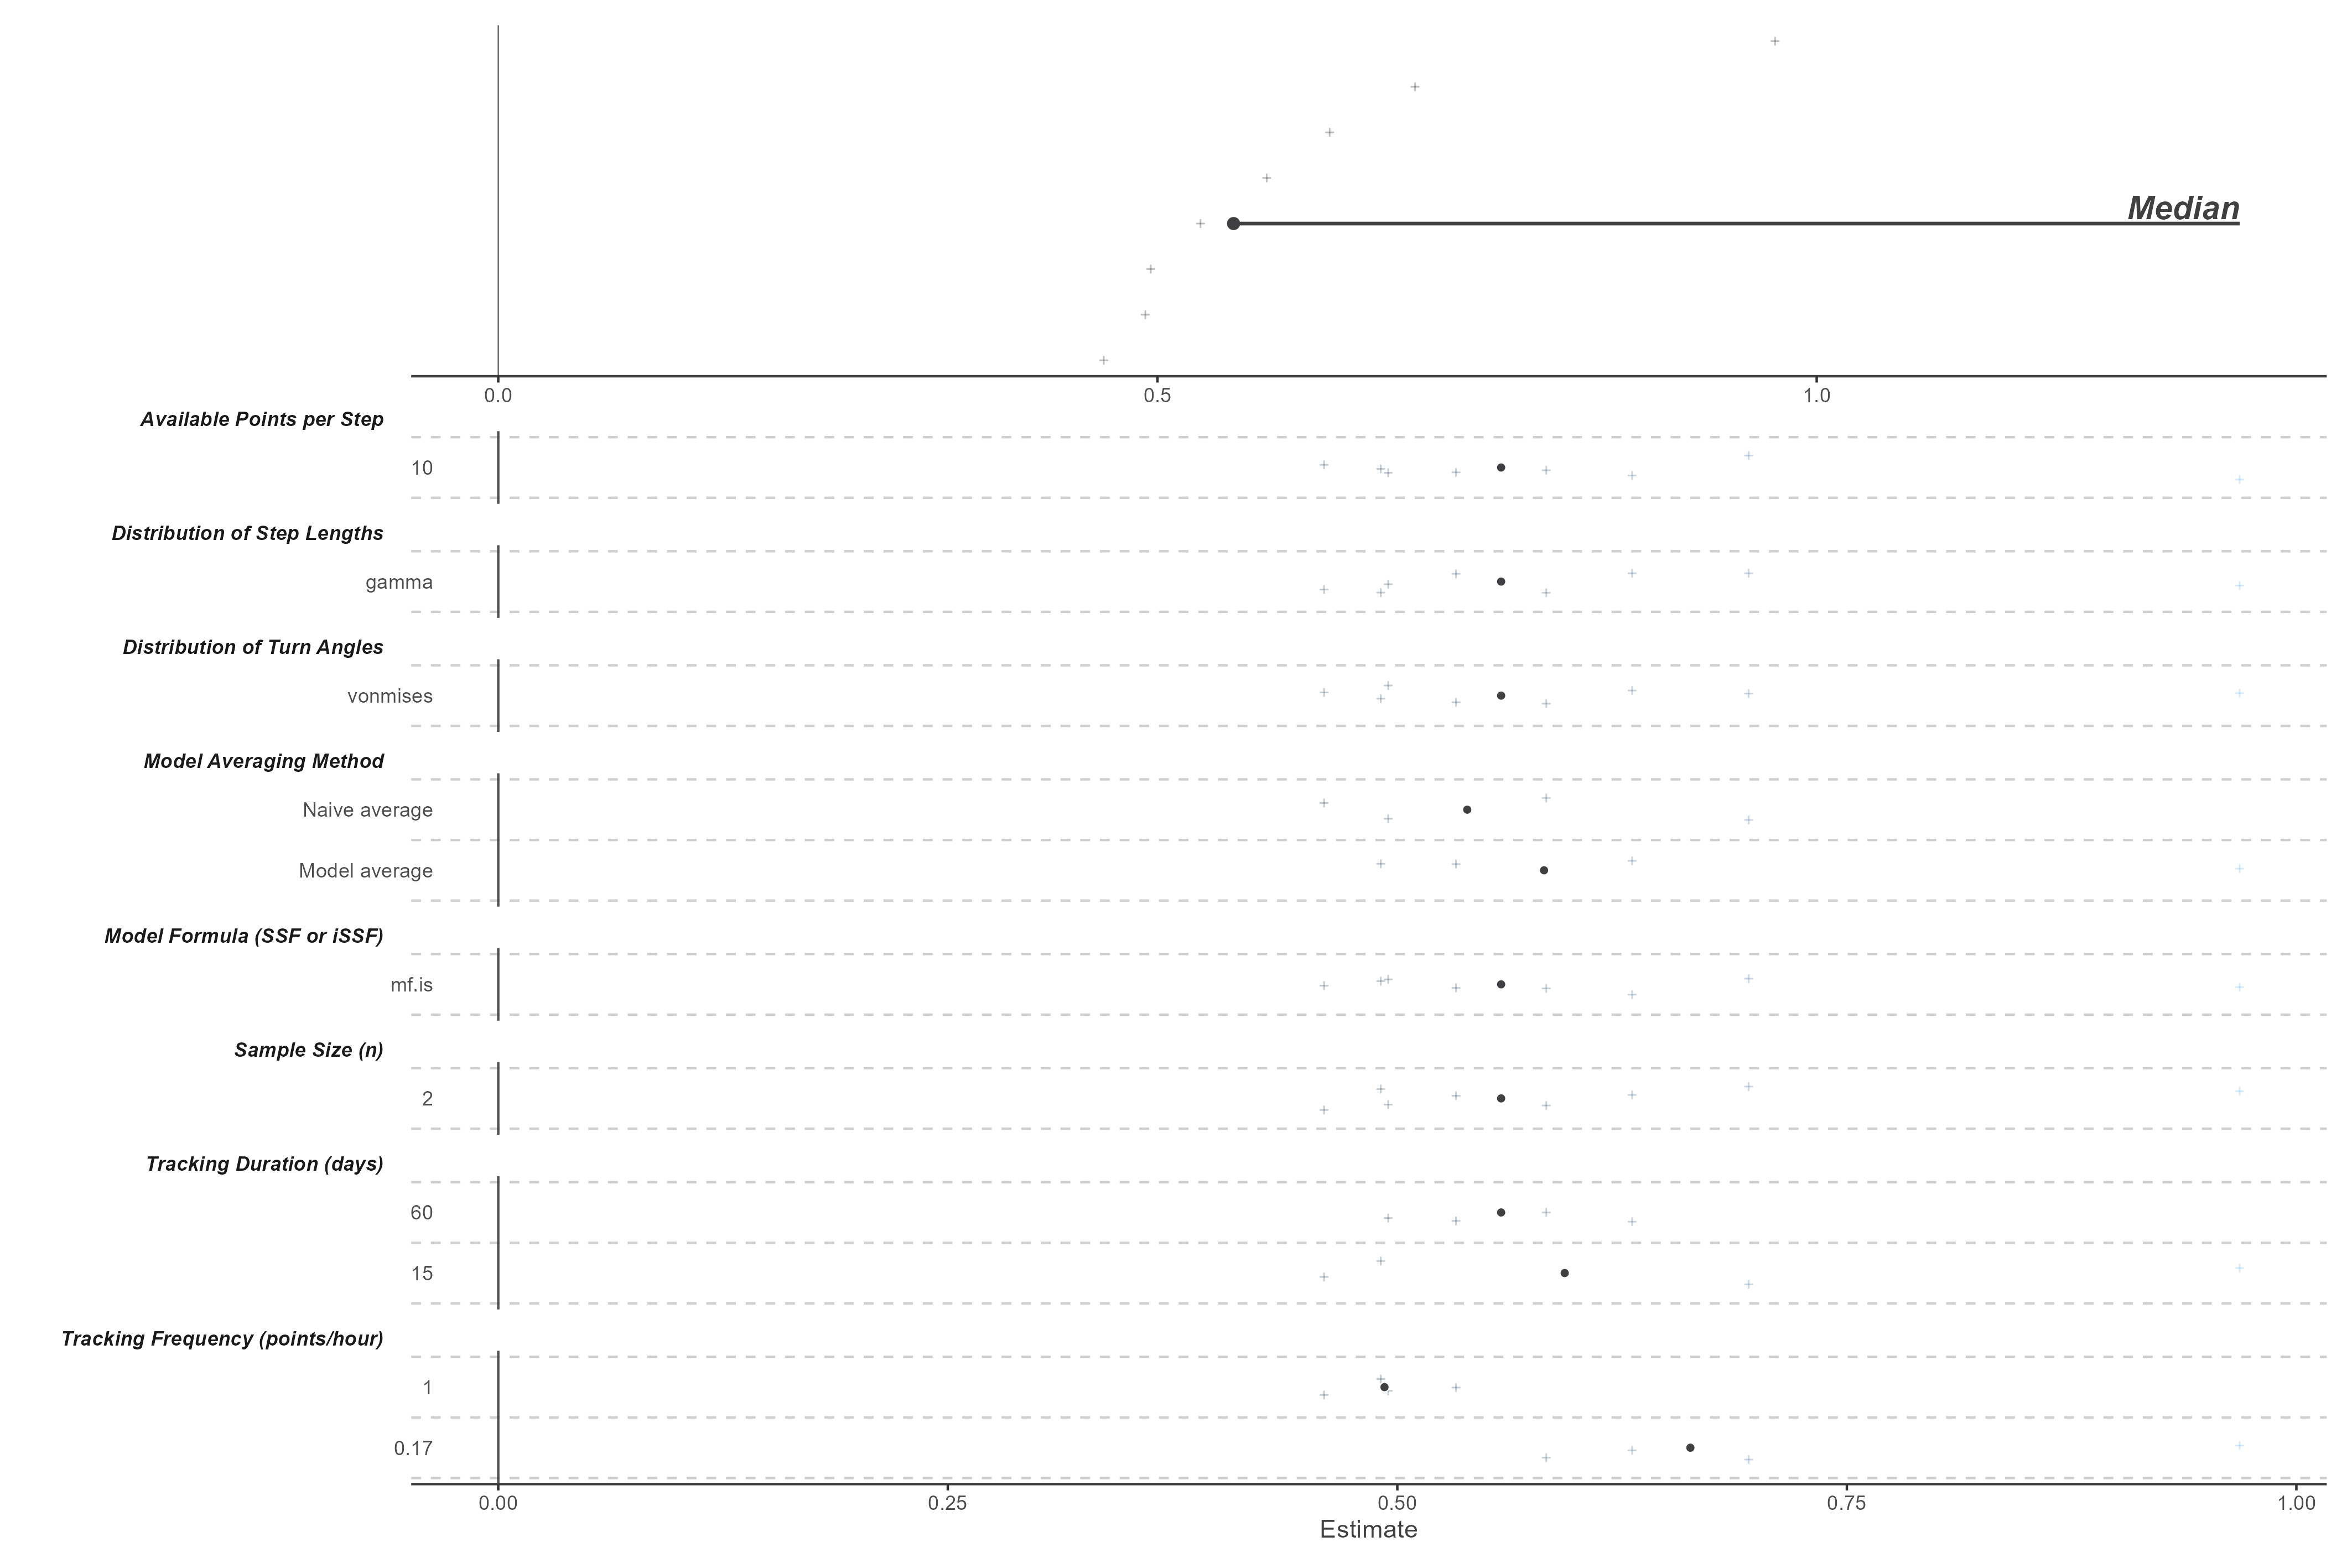
\includegraphics[width=1\linewidth]{../figures/ssf_specCurve} \caption{Spec curve}\label{fig:specCurveSSF}
\end{figure}

(Fig. \ref{fig:specCurvePois}).

\begin{figure}
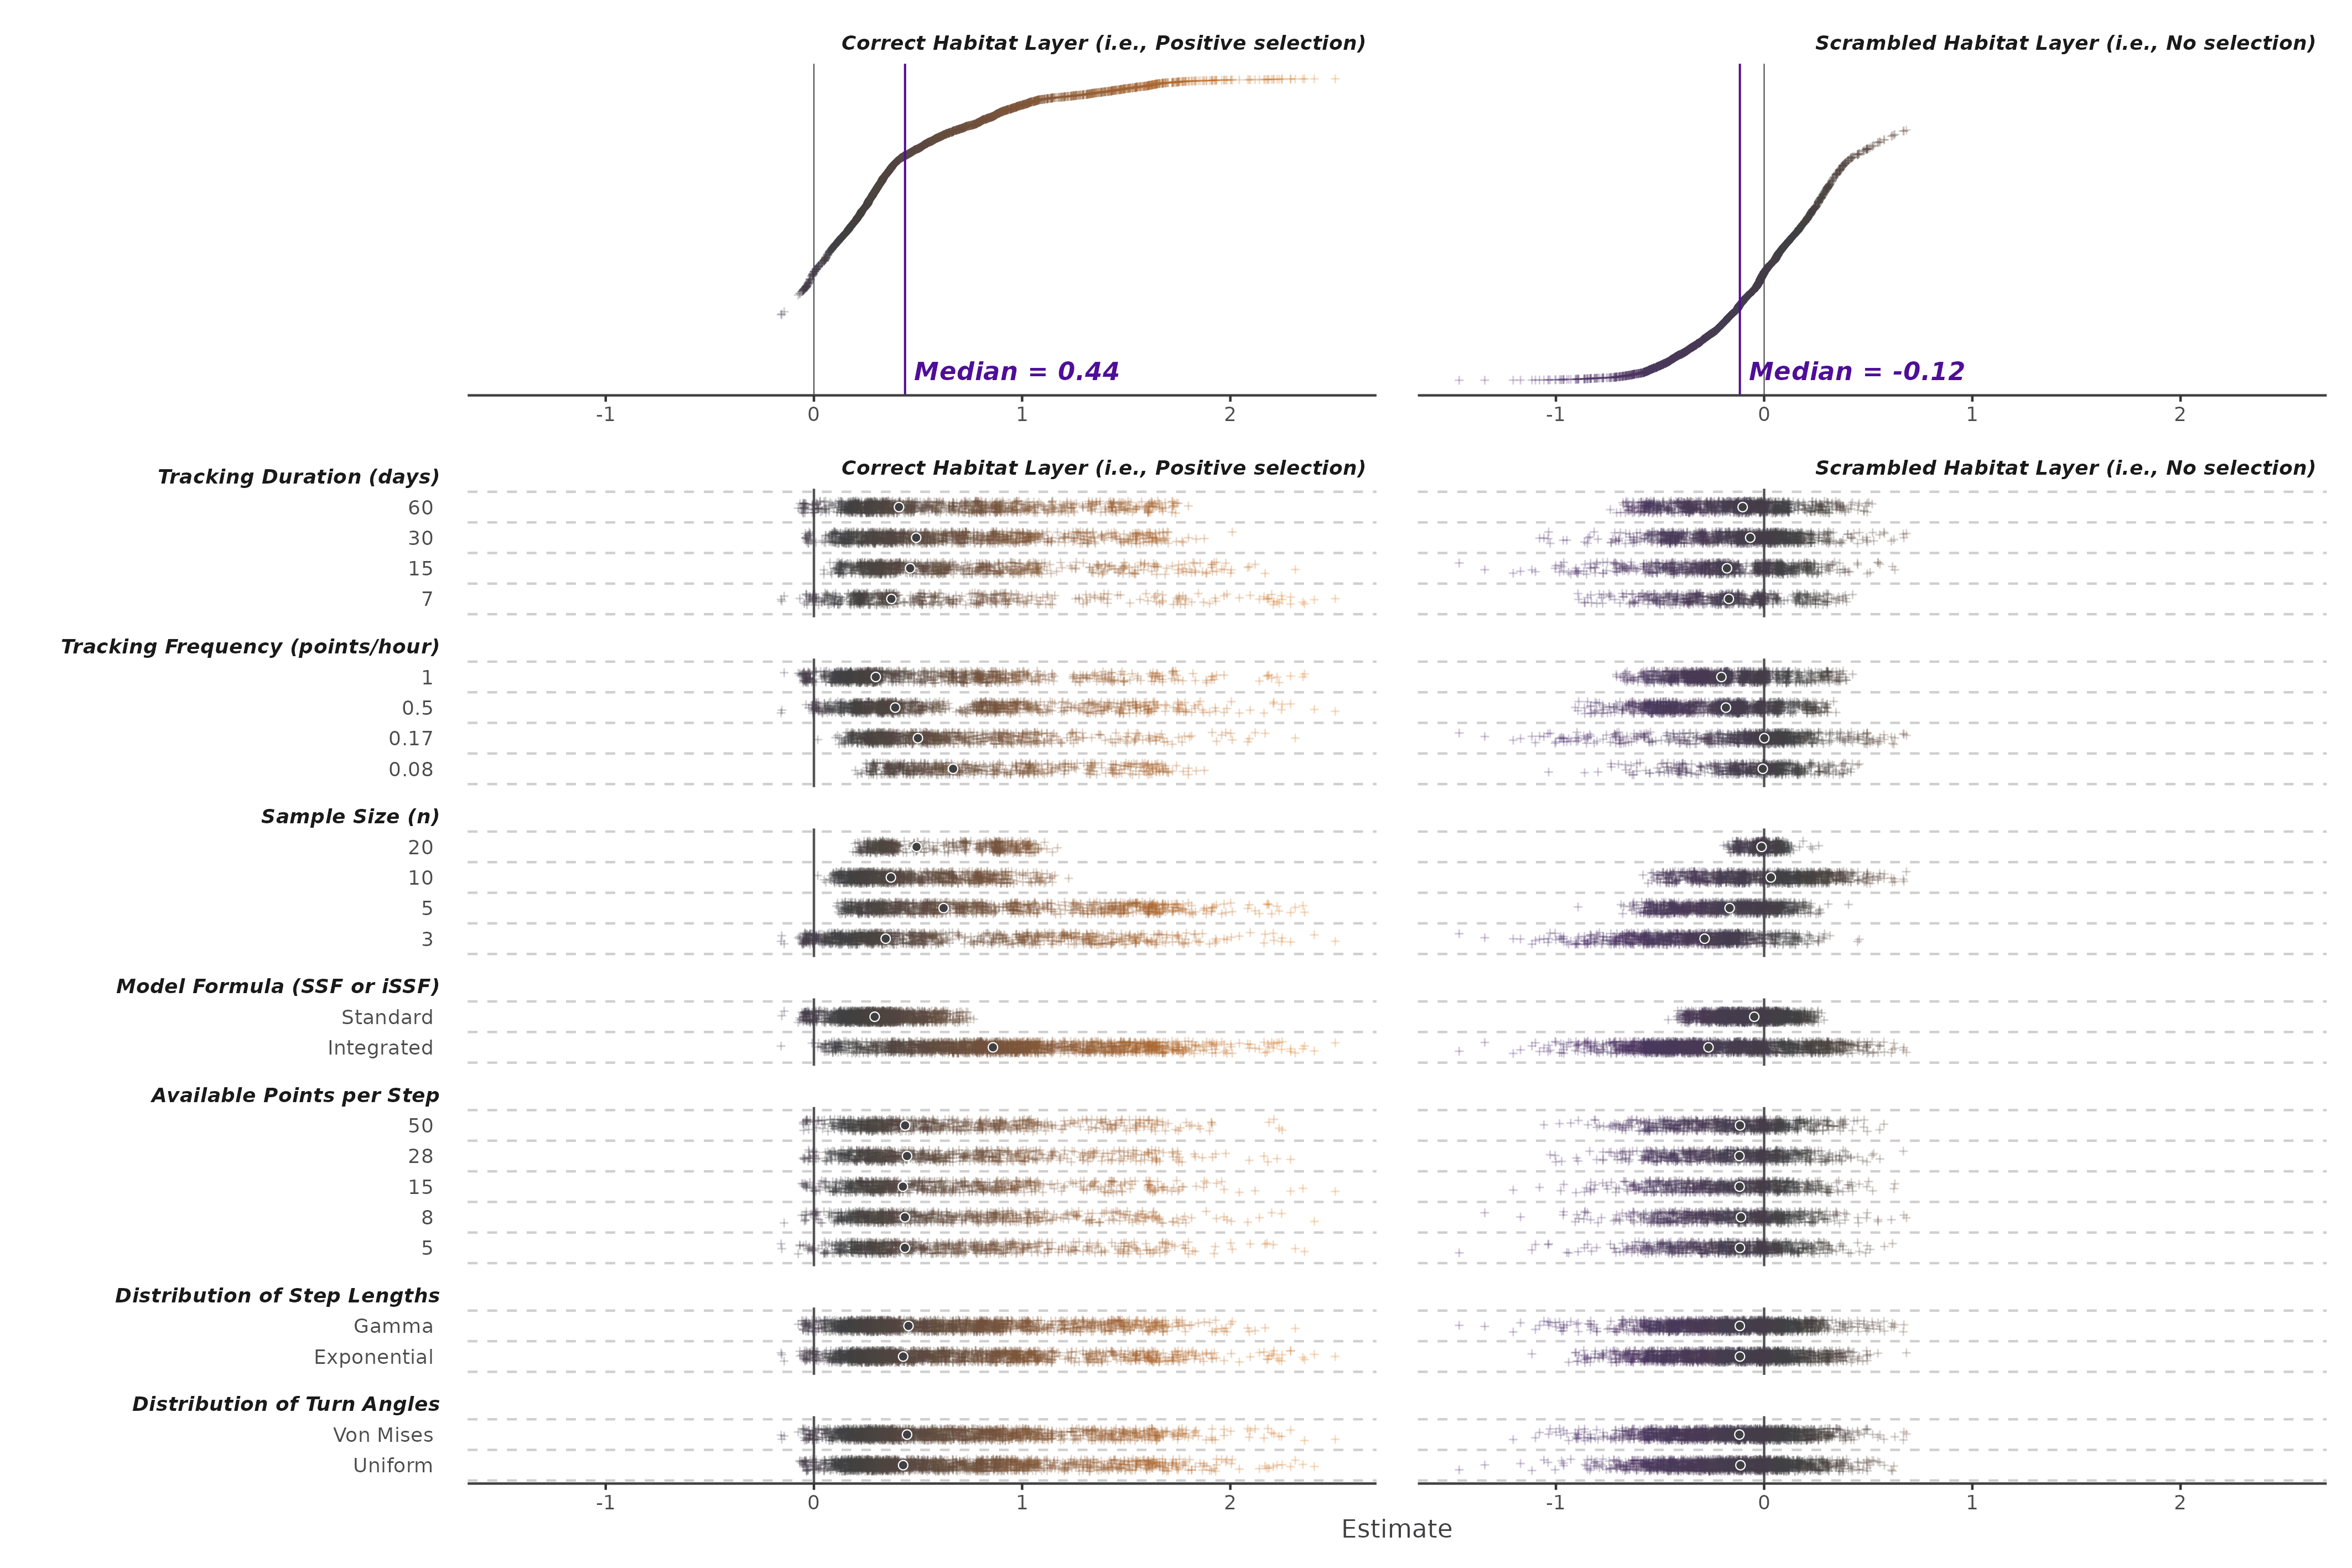
\includegraphics[width=1\linewidth]{../figures/pois_specCurve} \caption{Spec curve}\label{fig:specCurvePois}
\end{figure}

\hypertarget{model-results}{%
\subsection{Model Results}\label{model-results}}

The conditional \emph{R\textsuperscript{2}} values differed for the three models. The Compana results model had a conditional \emph{R\textsuperscript{2}} of 0.33; whereas the SSF model returned 0.59, and the Poisson model returned 0.94.

The marginal \emph{R\textsuperscript{2}} represents the bulk of the conditional \emph{R\textsuperscript{2}} suggesting an important role for the fixed/population effects. The Compana results model had a conditional \emph{R\textsuperscript{2}} of 0.48; whereas the SSF model returned 0.51, and the Poisson model returned 0.83.

The sample size was negatively correlated with deviation from the median estimate (\(\beta\) -0.03; 95\% HDCI -1.15 --- 1.8).

(Fig. \ref{fig:effectPlotArea}).

\begin{figure}
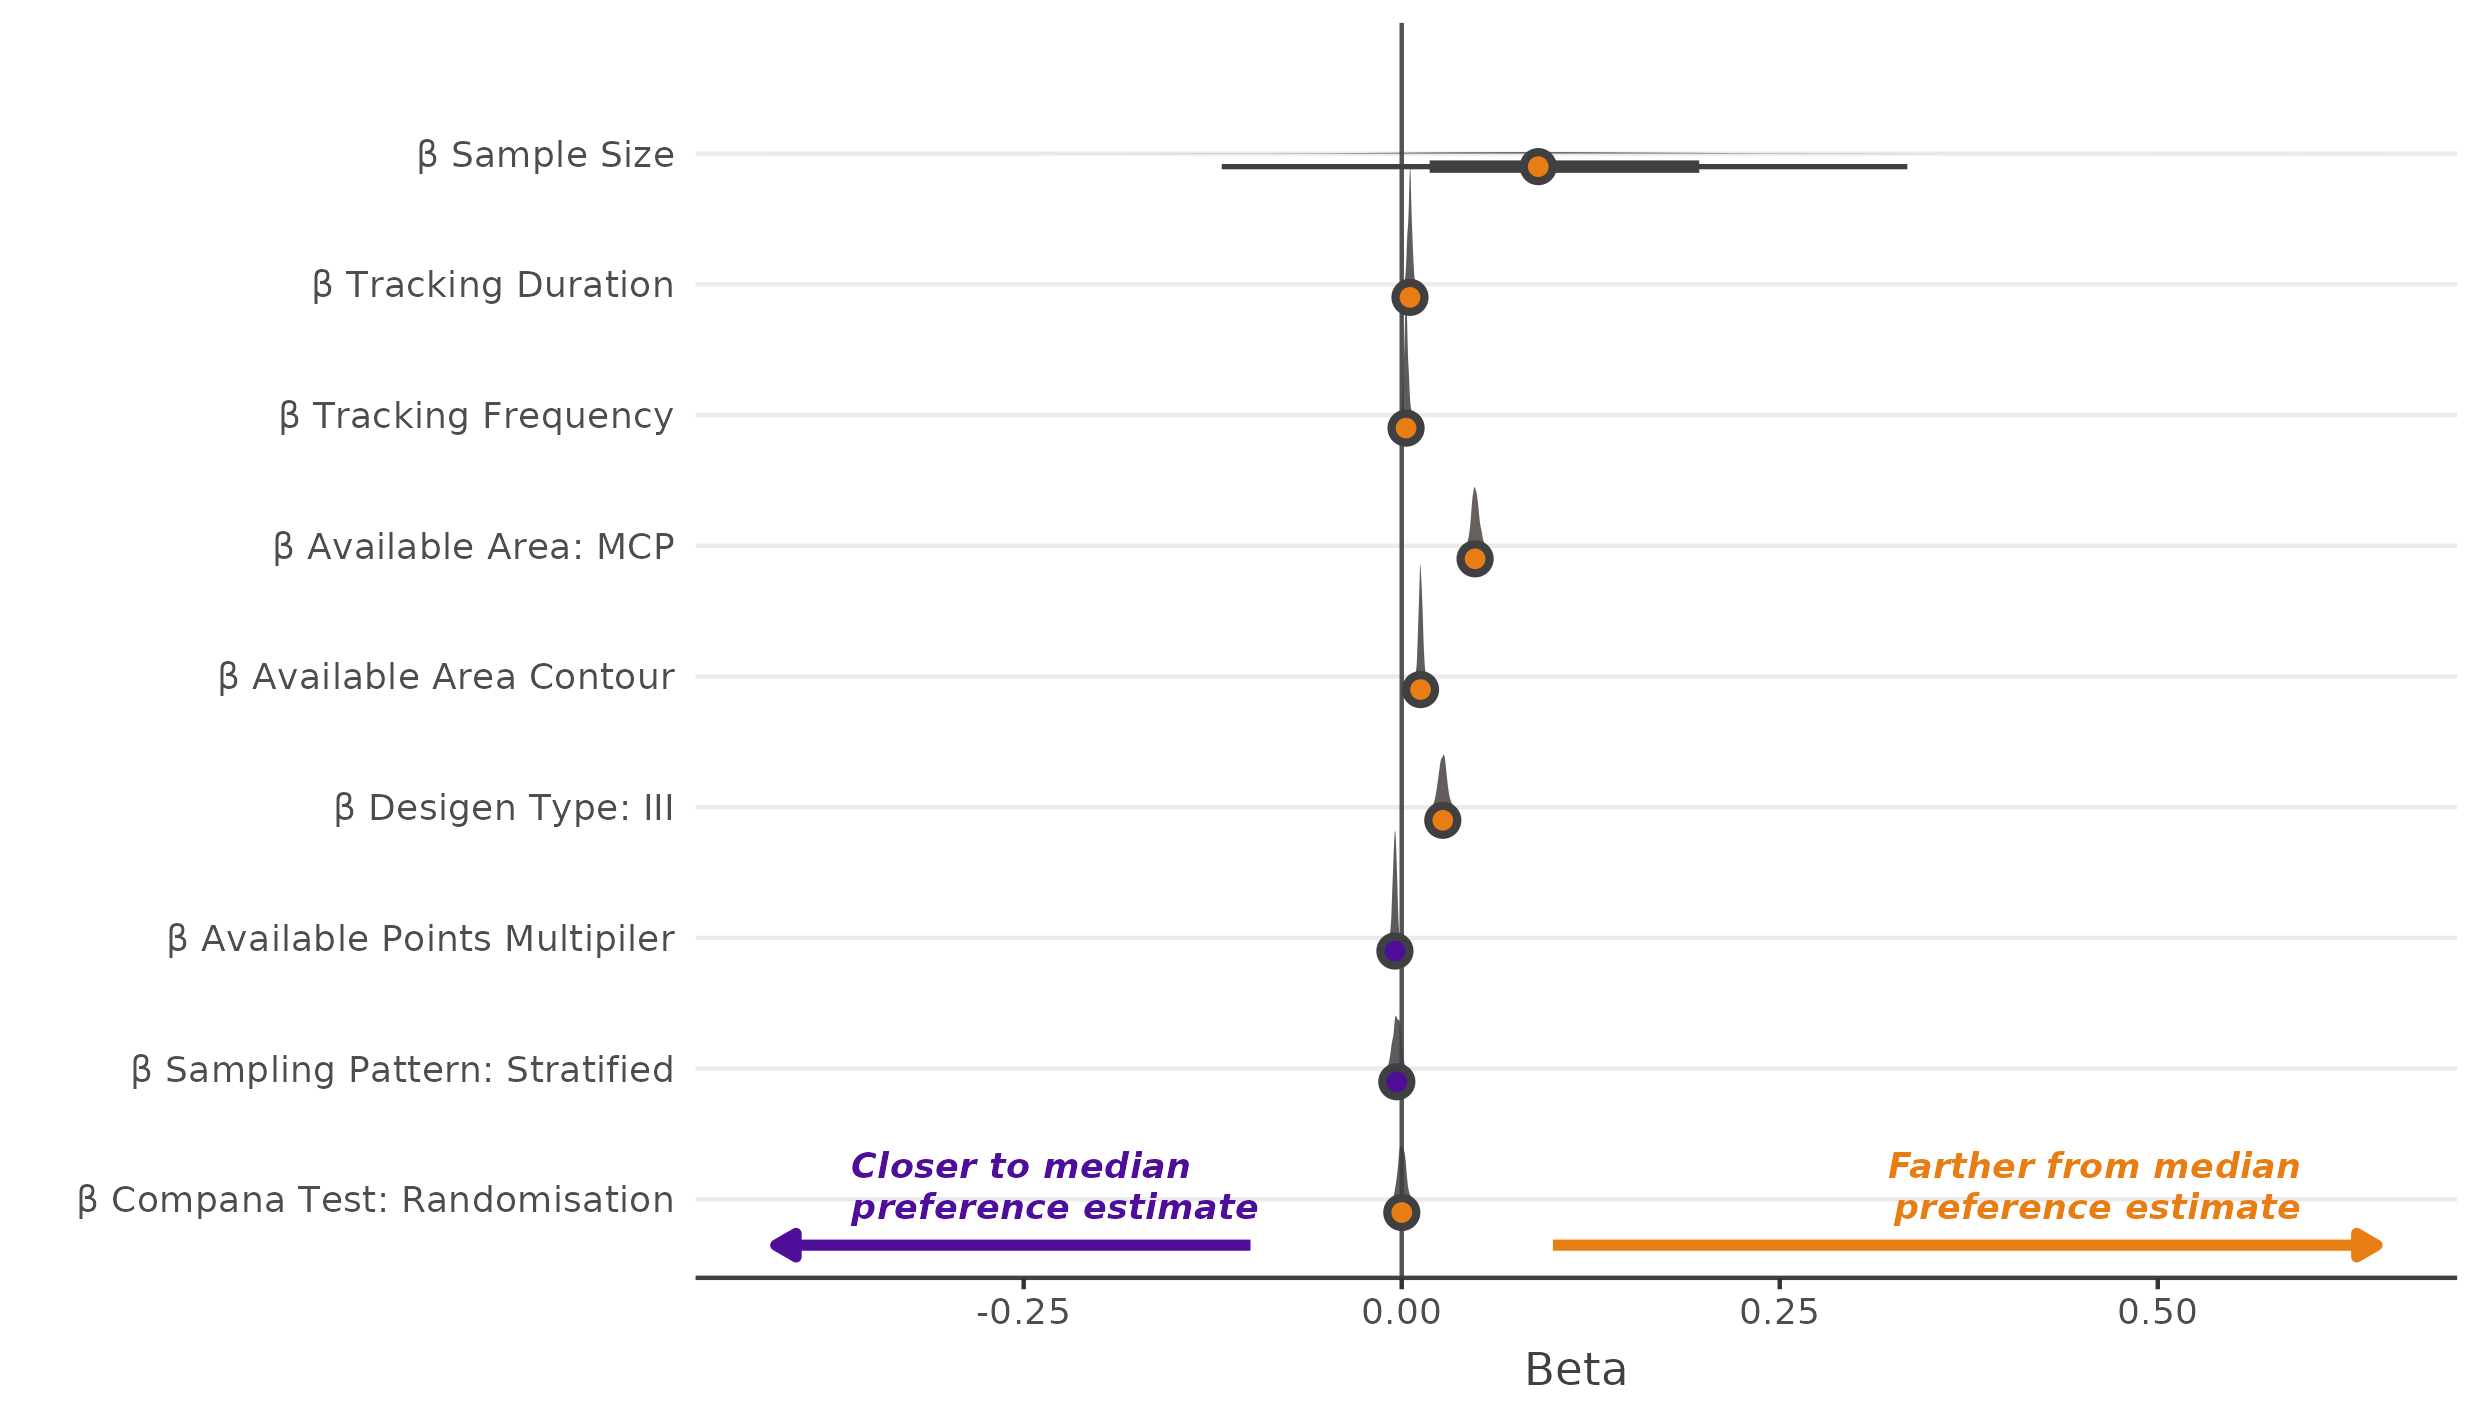
\includegraphics[width=1\linewidth]{../figures/areaBrms_effectsPlot} \caption{Beta coefs}\label{fig:effectPlotArea}
\end{figure}

(Fig. \ref{fig:effectPlotSSF}).

\begin{figure}
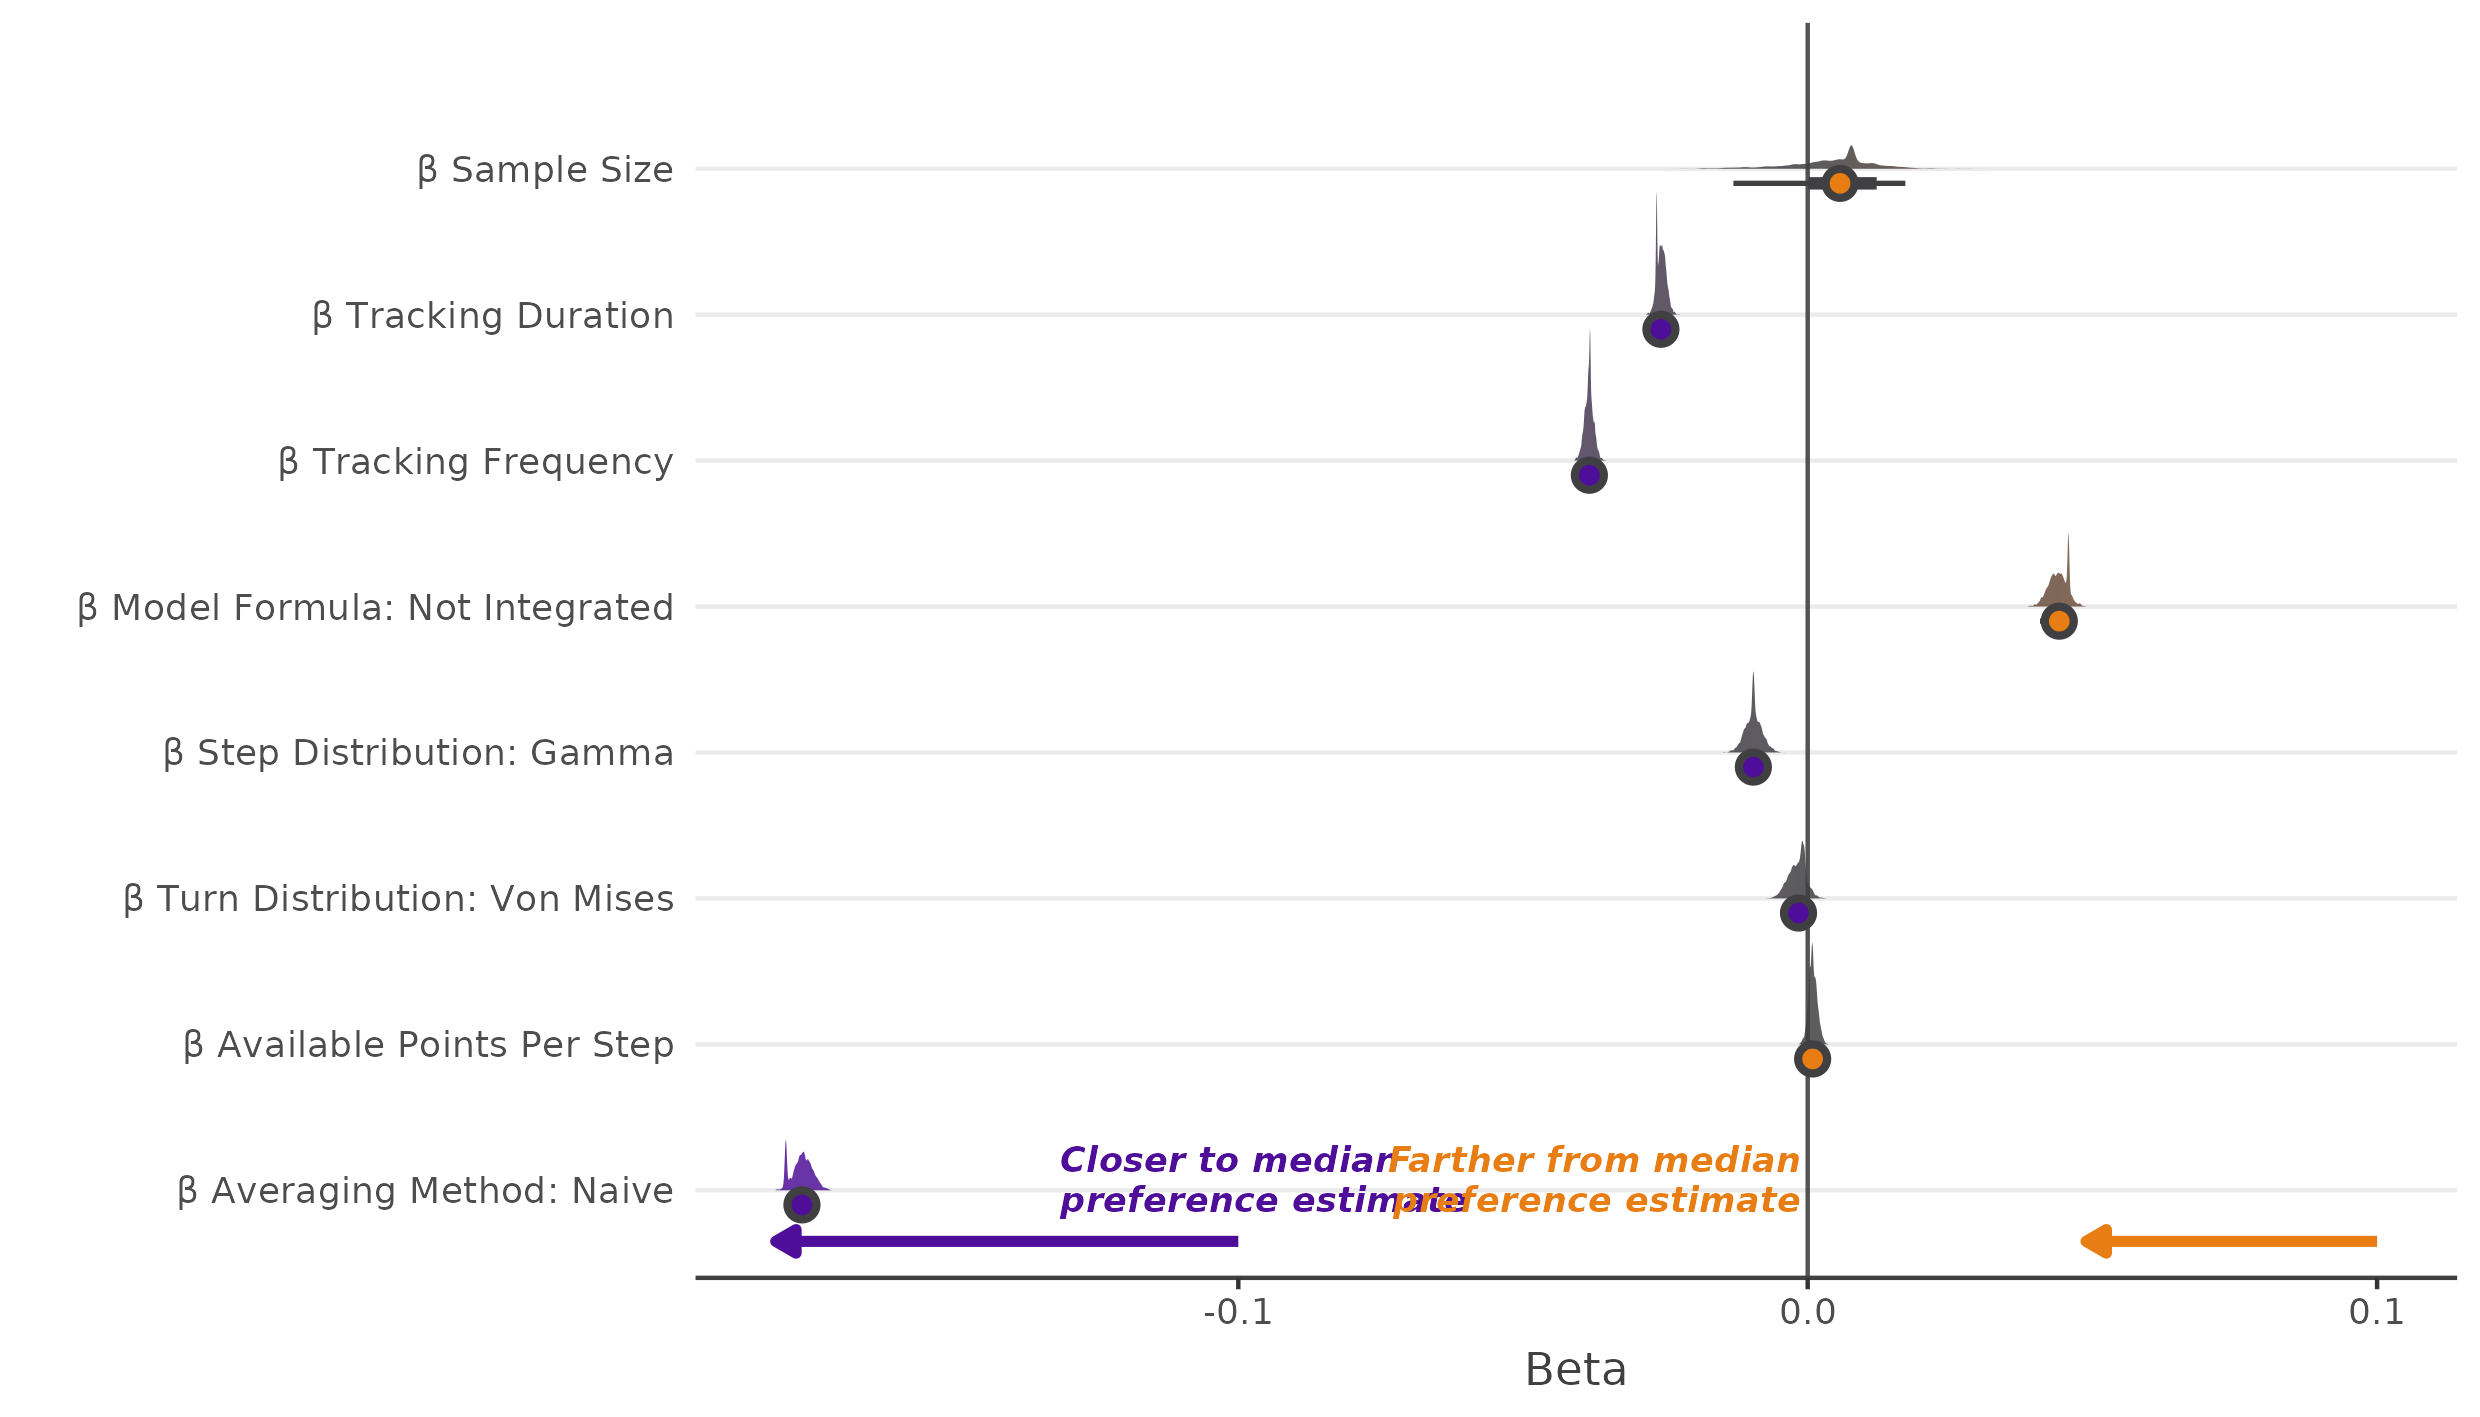
\includegraphics[width=1\linewidth]{../figures/ssfBrms_effectsPlot} \caption{Beta coefs}\label{fig:effectPlotSSF}
\end{figure}

(Fig. \ref{fig:effectPlotPois}).

\begin{figure}
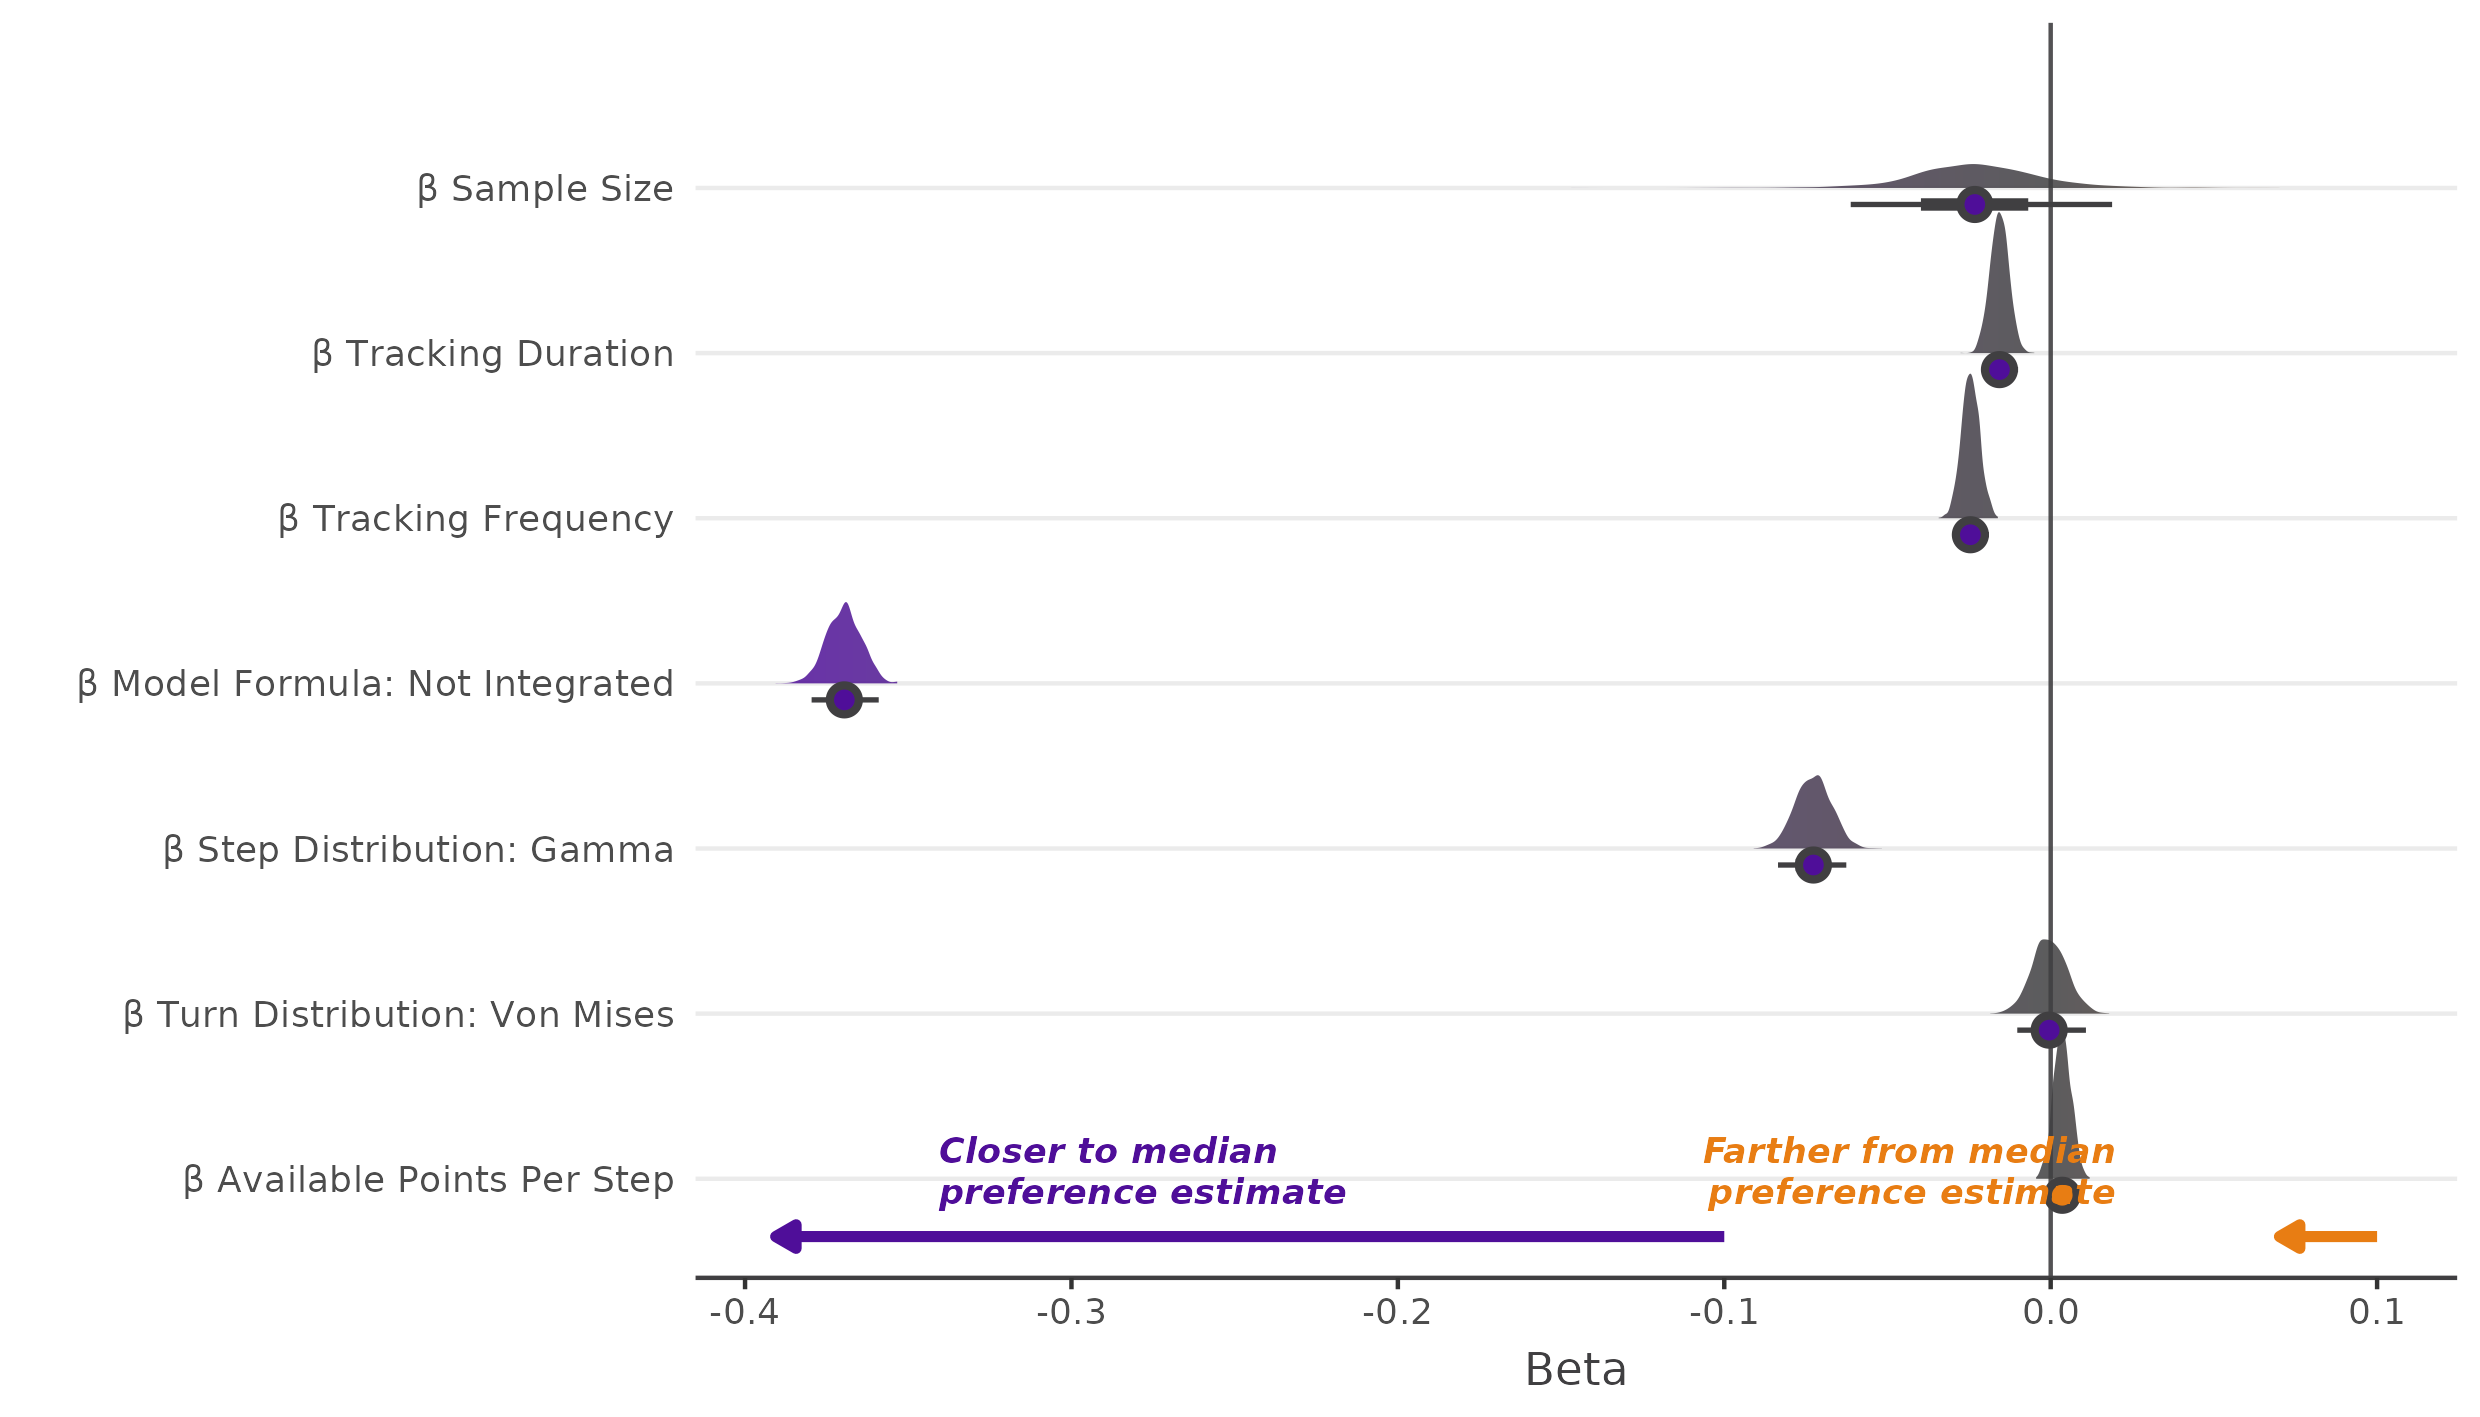
\includegraphics[width=1\linewidth]{../figures/poisBrms_effectsPlot} \caption{Beta coefs}\label{fig:effectPlotPois}
\end{figure}

\hypertarget{discussion}{%
\section{Discussion}\label{discussion}}

\end{document}
